\chapter{State of the Art in Optimal V2G Management}

\section{The V2G Imperative: A Cornerstone of Europe's Green Transition}
Our society stands at a critical juncture, facing the twin revolutions of decarbonizing transport and transforming our energy systems. This is not merely an ambition but a legally binding mandate, enshrined in frameworks like the \textbf{European Green Deal} and its ambitious \textbf{"Fit for 55"} package \footcite{european_commission_2021_fit_for_55}. These policies impose a rapid phase-out of internal combustion engines and mandate a massive scale-up of renewable energy sources, as detailed in the revised Renewable Energy Directive (RED III) \footcite{RED_III_directive_2023}. The proliferation of Electric Vehicles (EVs) sits squarely at the nexus of this challenge.
\\
\noindent
Initially viewed with apprehension—a looming threat of massive, synchronized loads poised to destabilize fragile distribution networks—that perception is now obsolete. Today, we must see EVs not as a problem, but as a foundational pillar of the solution. This paradigm shift is embodied in the concept of \textbf{Vehicle-to-Grid (V2G)}. V2G is the critical enabling technology that transforms millions of EVs from passive energy consumers into an active, distributed, and intelligent grid asset. The key lies hidden in plain sight: private vehicles remain parked and connected for an astonishing 96\% of their existence \footcite{evertsson2024investigating}, representing a potential of terawatt-hours of mobile storage waiting to be harnessed.
\\
\noindent
The true power of V2G is not in the individual, but in the collective. A single EV's contribution is a whisper, but a coordinated fleet, managed by an aggregator, becomes a roar—a \textbf{Virtual Power Plant (VPP)}. This collective entity, with the lightning-fast response of battery inverters, can deliver a spectrum of critical services. This capability is the linchpin for stabilizing a grid increasingly reliant on the fluctuating whims of wind and sun, making the high renewable penetration targets of the EU feasible. The services enabled are foundational to the smart, resilient grid of tomorrow:
\begin{itemize}
    \item \textbf{Frequency Regulation:} The grid's heartbeat. V2G fleets can inject or absorb power in seconds, instantly counteracting supply-demand imbalances to maintain the stable 50/60 Hz frequency, preventing cascading failures and blackouts \footcite{alfaverh2022optima, sadeghi2021deep}.
    
    \item \textbf{Demand Response and Peak Shaving:} By intelligently shifting charging to off-peak hours and discharging during peak demand, V2G flattens the load curve. This reduces our reliance on expensive and polluting "peaker" plants and can defer trillions in grid infrastructure upgrades \footcite{orfanoudakis2022deep}.
    
    \item \textbf{Renewable Energy Integration:} Perhaps the most profound impact. V2G fleets act as a giant, distributed sponge, absorbing surplus solar and wind energy that would otherwise be curtailed and wasted, and releasing it when the sun sets or the wind dies down. This directly supports the integration goals of RED III and mitigates intermittency \footcite{khan2024review, zou2021deep}.
\end{itemize}
This vision is no longer a distant prospect but is actively being codified into European law and technical standards. The landmark \textbf{Alternative Fuels Infrastructure Regulation (AFIR, EU 2023/1804)} now mandates that new public charging infrastructure must support smart and bidirectional charging capabilities. This legal requirement is given its technical teeth by specific standards; a delegated regulation specifies that from 2027, charging points must comply with \textbf{ISO 15118-20}, a standard that explicitly defines the communication protocols for bidirectional power transfer. This regulatory push is complemented by large-scale pilot projects like \textbf{'SCALE'} and \textbf{'V2G Balearic Islands'}, which are testing the technology's technical and economic viability on an industrial scale.
\\
\noindent
However, while the regulatory foundation is being laid, significant barriers to widespread adoption remain, creating a complex landscape that technology and policy must navigate together. Key challenges include:
\begin{itemize}
    \item \textbf{Market and Economic Hurdles:} A clear, pan-European framework for remunerating EV owners for grid services is still absent. Critical issues like the \textbf{"double taxation"} of electricity—taxed both on charging and discharging—create significant economic disincentives and must be resolved.
    \item \textbf{Regulatory and Grid Access Rules:} The role of EV fleets as a flexibility resource is not yet uniformly recognized in electricity markets. Standardized procedures for grid connection, aggregator certification, and secure data exchange are still under development, hindering market access.
    \item \textbf{Technical and Consumer Barriers:} On the consumer side, concerns about accelerated \textbf{battery degradation} and its impact on vehicle warranties remain a primary obstacle. Furthermore, the reality is that not all EVs or chargers are currently equipped with the necessary hardware and software to support V2G.
\end{itemize}
Therefore, the central challenge—and the focus of this thesis—is not merely to enable V2G, but to do so \textit{intelligently}. It requires a control strategy sophisticated enough to operate within this nascent regulatory framework, navigate its economic uncertainties, and overcome technical constraints to unlock the immense potential of EVs as a cornerstone of a sustainable energy future.

%%%%%%%%%%%%%%%%%
\section{The Optimizer's Trilemma: Navigating a Stochastic World}
While the potential is immense, orchestrating this symphony of distributed assets is a formidable challenge. The primary driver for an aggregator is economic viability, but pursuing profit in isolation is a recipe for failure. Optimal V2G management is a delicate balancing act, a genuine multi-objective optimization problem often framed as the "V2G trilemma": the simultaneous pursuit of \textbf{economic profitability}, the preservation of \textbf{battery longevity}, and the guarantee of \textbf{user convenience}.
\\
\noindent
This is not a simple trade-off. It is a dynamic problem steeped in \textbf{stochasticity} and \textbf{uncertainty} from multiple sources:
\begin{itemize}
    \item \textbf{Market Volatility:} Electricity prices can fluctuate wildly based on unpredictable supply and demand.
    \item \textbf{Renewable Intermittency:} The output of solar and wind generation is inherently variable.
    \item \textbf{Human Behavior:} EV owners' arrival times, departure times, and energy needs are not deterministic; a driver might need to leave unexpectedly, a non-negotiable constraint that any intelligent system must respect.
\end{itemize}
This chaotic environment renders static, rule-based control systems obsolete. We need an approach that can learn, adapt, and make intelligent decisions in real-time under profound uncertainty. This is precisely the domain of Reinforcement Learning.

\section{A New Paradigm for Control: Reinforcement Learning}
To tackle the V2G challenge, we turn to Reinforcement Learning (RL), a field of machine learning concerned with how an intelligent agent learns to make optimal decisions through trial and error. Unlike traditional methods that require a perfect model of the world, RL learns directly from interaction, making it exceptionally robust.

\subsection{The Language of Learning: Markov Decision Processes (MDPs)}
The mathematical foundation of RL is the \textbf{Markov Decision Process (MDP)}, formally defined by the tuple $(S, A, p, R, \gamma)$. In the V2G context:
\begin{itemize}
    \item $S$ is the state (a snapshot of the world: battery levels, electricity price, time).
    \item $A$ is the action (the decision: the charging/discharging rate for each EV).
    \item $p(s',r|s,a)$ is the environment's response (the probability of transitioning to a new state $s'$ and receiving reward $r$).
    \item $R$ is the reward (the feedback signal: profit generated, penalty for user dissatisfaction).
    \item $\gamma$ is the discount factor, balancing immediate vs. future rewards.
\end{itemize}
This framework rests on the \textbf{Markov Property}, which allows the agent to make decisions based solely on the current state.

\subsection{Judging the Future: Value Functions and Actor-Critic Architectures}
The agent's goal is to learn a \textbf{policy}, $\pi(a|s)$, a strategy for choosing actions. To do this, it learns \textbf{value functions}, which estimate the long-term value of being in a certain state ($v_{\pi}(s)$) or taking a specific action in a state ($q_{\pi}(s, a)$).
\\
\noindent
The \textbf{Actor-Critic} architecture provides an elegant way to learn the policy. It maintains two distinct components:
\begin{itemize}
    \item \textbf{The Critic}: It learns the value function. Its job is to evaluate the actor's decisions.
    \item \textbf{The Actor}: It is the policy. Its job is to select actions, using the critic's feedback to improve its strategy over time.
\end{itemize}
This architecture is particularly powerful for V2G because it can directly learn a policy over a continuous action space, allowing for precise control of power. The agent's entire behavior, however, is shaped by the reward signal it receives. The complex art of designing this signal to align the agent's goals with our multi-faceted objectives is a critical discipline in itself, known as reward engineering.

% ===================================================================
% REWARD SHAPING SECTION
% The detailed discussion on reward shaping techniques (PBRS, Dynamic,
% Curriculum Learning) is now encapsulated in the external file.
% ===================================================================
\section{Reward Engineering: Shaping Agent Behavior}
\label{sec:reward_shaping}

The reward function is arguably the most critical component in a Reinforcement Learning system. It is the sole mechanism through which a designer can communicate the desired behavior to the agent. A poorly designed reward can lead to unintended and suboptimal behaviors, even if the agent successfully maximizes it. The entire field of reward engineering has become a cornerstone of modern RL, as it is fundamental to applying these algorithms effectively in complex, real-world applications \footcite{ibrahim2024comprehensive}. The V2G problem, with its multiple competing objectives—maximizing profit, ensuring user satisfaction, preserving battery health, and maintaining grid stability—makes reward design particularly challenging. This work explores several sophisticated techniques to guide the learning process effectively.

\subsection{Potential-Based Reward Shaping (PBRS)}
Potential-Based Reward Shaping (PBRS) is perhaps the most theoretically sound method for reward augmentation \footcite{ng1999policy}. It involves adding a shaping term, $F(s, s')$, to the environment's intrinsic reward, $R(s, a, s')$. The new, shaped reward $R'$ is thus defined as:
\[
R'(s, a, s') = R(s, a, s') + F(s, s')
\]
The shaping term itself is defined as the difference between a potential function, $\Phi$, evaluated at the new state and the old state:
\[
F(s, s') = \gamma \Phi(s') - \Phi(s)
\]
where $\gamma$ is the discount factor. The key theoretical guarantee of PBRS is \textbf{policy invariance}: adding a potential-based shaping reward does not change the optimal policy of the underlying MDP. While the agent learns the same optimal behavior, the shaping term can provide dense, intermediate rewards that significantly accelerate the learning process by guiding the agent's exploration.

\subsection{Dynamic and Adaptive Rewards}
Unlike PBRS, which provides a static reward bonus, a dynamic or adaptive reward function can evolve during training. This approach is particularly useful for complex problems where the relative importance of different objectives may change as the agent becomes more competent. For example, an agent could initially be rewarded simply for keeping an EV charged, but as training progresses, the reward function could adapt to introduce penalties for grid overloads or incentives for V2G services \footcite{wan2022dynamic}. This allows the agent to master different facets of the problem sequentially.

\subsection{Curriculum Learning}
While technically a training paradigm rather than a reward modification technique, Curriculum Learning (CL) is highly relevant to reward engineering. CL involves training the agent on a sequence of tasks that gradually increase in difficulty. In the V2G context, an agent might first be trained in a simple scenario with only a few EVs and stable prices. Once it masters this, it is moved to a more complex environment with more EVs, volatile prices, and hard constraints. This structured learning process prevents the agent from being overwhelmed by the full complexity of the problem from the start and can lead to more robust and generalizable policies.


\section{The Rise of Deep Reinforcement Learning for V2G Control}
The fusion of RL with the representational power of deep neural networks gives us \textbf{Deep Reinforcement Learning (DRL)}, the state-of-the-art paradigm for V2G control. The journey of DRL algorithms applied to V2G is one of increasing sophistication and robustness, branching into two main families: off-policy and on-policy methods, each with its own philosophy and set of trade-offs.

\subsection{Off-Policy Methods: Data-Efficient Learning from Experience}
Off-policy algorithms are characterized by their ability to learn the optimal policy from data generated by a different, often more exploratory, policy. This decoupling allows them to reuse past experiences stored in a \textit{replay buffer}, making them highly sample-efficient and well-suited for complex problems where real-world interaction is costly.

\paragraph{Deep Deterministic Policy Gradient (DDPG)}
A seminal algorithm that extended the success of Deep Q-Networks (DQN) to continuous action spaces, DDPG was a foundational breakthrough for control problems like V2G\footcite{lillicrap2015continuous}. As an Actor-Critic method, it learns a deterministic policy (the Actor) that maps states to specific actions, guided by a Q-value function (the Critic). However, its practical application is often hindered by training instability and a crippling vulnerability to \textbf{overestimation bias}, where the Critic systematically overestimates Q-values. This error propagates through the learning process, causing the Actor to converge on suboptimal policies\footcite{orfanoudakis2022deep, alfaverh2022optima}.

\paragraph{Twin Delayed DDPG (TD3)}
TD3 was developed specifically to address the instabilities of DDPG\footcite{fujimoto2018addressing}. It introduces three crucial innovations:
\begin{enumerate}
    \item \textbf{Clipped Double Q-Learning:} It learns two independent Critic networks and uses the minimum of their Q-value predictions to calculate the target value. This conservative approach effectively mitigates the overestimation bias.
    \item \textbf{Delayed Policy Updates:} The Actor and target networks are updated less frequently than the Critic. This allows the Critic's value estimate to stabilize before the policy is modified, leading to smoother and more reliable training.
    \item \textbf{Target Policy Smoothing:} A small amount of clipped noise is added to the target action, which helps to regularize the learning process and prevent the policy from exploiting narrow peaks in the value function.
\end{enumerate}
These additions make TD3 a much more robust and reliable baseline for V2G tasks\footcite{liu2023optimal, wang2022multi}.

\paragraph{Soft Actor-Critic (SAC)}
SAC represents the current state-of-the-art for continuous control, offering superior sample efficiency and stability\footcite{haarnoja2018soft}. Its core innovation is the \textbf{maximum entropy framework}. The agent's objective is not just to maximize the cumulative reward, but to do so while acting as randomly (stochastically) as possible. This entropy bonus encourages broad exploration, preventing premature convergence to a narrow, suboptimal policy, and improves robustness by learning to "keep its options open"\footcite{logeshwaran2022comparative}.

\paragraph{Truncated Quantile Critics (TQC)}
TQC tackles overestimation bias from a distributional perspective, offering a more fundamental solution than TD3\footcite{kuznetsov2020controlling}. Instead of learning a single expected return (Q-value), it learns the entire \textit{distribution of returns} by using quantile regression with multiple Critic networks. Its key mechanism is to "truncate" (discard) the top-k most optimistic quantile estimates when forming the target distribution, thereby systematically removing the primary source of overestimation bias.

\paragraph{Enhancement: Prioritized Experience Replay (PER)}
This is not a standalone algorithm but a crucial modification for off-policy methods. Instead of sampling uniformly from the replay buffer, PER samples transitions with a probability proportional to their "importance," measured by the magnitude of their TD error. This focuses the learning process on "surprising" or informative experiences, significantly accelerating convergence\footcite{schaul2015prioritized}.

\subsection{On-Policy Methods: Stability through Cautious Updates}
On-policy methods learn from data generated exclusively by the current policy. This means that after each policy update, all previously collected data must be discarded. While this makes them inherently less sample-efficient, their updates are often more stable and less prone to divergence.

\paragraph{Advantage Actor-Critic (A2C/A3C)}
A2C is a foundational on-policy Actor-Critic algorithm. Its practical and powerful extension, \textbf{Asynchronous Advantage Actor-Critic (A3C)}, uses parallel workers to interact with multiple copies of the environment. These workers update a global set of parameters asynchronously, which decorrelates the data stream and provides a powerful stabilizing effect on the learning process\footcite{mnih2016asynchronous}.

\paragraph{Trust Region Policy Optimization (TRPO)}
TRPO was the first algorithm to rigorously formalize the idea of controlling the policy update size to guarantee stable, monotonic improvements\footcite{schulman2015trust}. It maximizes a surrogate objective function subject to a constraint on the "behavioral change" of the policy, measured by the Kullback-Leibler (KL) divergence. This creates a "trust region" around the old policy, preventing catastrophic updates that could destroy performance. However, its implementation is complex as it requires second-order optimization.

\paragraph{Proximal Policy Optimization (PPO)}
PPO achieves the stability benefits of TRPO using only first-order optimization, making it much simpler to implement and more widely applicable\footcite{schulman2017proximal}. Instead of a hard constraint, PPO modifies the objective function with a \textbf{clipping} mechanism that disincentivizes policy updates that result in a large probability ratio between the new and old policies. This creates a "soft" trust region and has become a default choice for many on-policy applications due to its robustness and ease of use.

\subsection{Gradient-Free Methods: An Alternative Path}
\paragraph{Augmented Random Search (ARS)}
ARS is an on-policy, gradient-free method that optimizes the policy by operating directly in the parameter space\footcite{mania2018simple}. Instead of calculating gradients, it explores random directions around the current policy parameters and updates them based on the observed performance. While often much less sample-efficient than gradient-based methods for complex V2G problems, its simplicity can be competitive in certain scenarios.


\section{A Comparative Perspective on Control Methodologies}
While DRL represents the cutting edge, it is crucial to contextualize it within the broader landscape.

\begin{table}[h!]
\centering
\caption{Comparative Analysis: DRL vs. Model Predictive Control (MPC) for V2G}
\label{tab:drl_vs_mpc}
\begin{tabular}{|p{0.2\linewidth}|p{0.35\linewidth}|p{0.35\linewidth}|}
\hline
\textbf{Aspect} & \textbf{Deep Reinforcement Learning (DRL)} & \textbf{Model Predictive Control (MPC)} \\ \hline
\textbf{Paradigm} & Model-Free, learning-based. Learns optimal policy via trial-and-error. & Model-Based, optimization-based. Solves an optimization problem at each step. \\ \hline
\textbf{Strengths} & \begin{itemize} \item Highly robust to uncertainty and stochasticity. \item No need for an explicit system model. \item Can learn complex, non-linear control policies. \item Fast inference time once trained. \end{itemize} & \begin{itemize} \item Explicitly handles hard constraints (safety guarantees). \item Proactive and anticipatory if forecasts are accurate. \item Well-established and understood. \end{itemize} \\ \hline
\textbf{Weaknesses} & \begin{itemize} \item Can be sample-inefficient during training. \item Lacks hard safety guarantees (an active research area). \item "Black box" nature can make policies hard to interpret. \end{itemize} & \begin{itemize} \item Performance is fundamentally tied to model and forecast accuracy. \item Computationally expensive at each time step (curse of dimensionality). \item Brittle to forecast errors and unmodeled dynamics. \end{itemize} \\ \hline
\textbf{V2G Suitability} & Excellent for dynamic, uncertain environments with complex trade-offs. & Good for problems with simple dynamics and reliable forecasts, but struggles with real-world V2G complexity. \\ \hline
\end{tabular}
\end{table}
\noindent
\textbf{Model Predictive Control (MPC)} is the most powerful model-based alternative \footcite{alsabbagh2022reinforcement}. Its primary strength is its ability to handle constraints. However, its performance is fundamentally shackled to the accuracy of its internal model and forecasts \footcite{faggio2023design}. In the V2G domain, creating an accurate model is nearly impossible due to non-linear battery dynamics, market volatility, and human unpredictability. Furthermore, solving the large-scale Mixed-Integer Linear Program (MILP) required at each time step becomes computationally intractable for large fleets \footcite{schwenk2022computationally}.
\\
\noindent
Other methods, such as \textbf{meta-heuristic algorithms} (e.g., genetic algorithms), are typically used for offline scheduling and lack the real-time responsiveness required for dynamic V2G control \footcite{ghosh2024optimal, kumar2024integration}.
\\
\noindent
In conclusion, the singular advantage of DRL is its inherent ability to learn and internalize the complex, non-linear trade-offs of the multi-objective V2G problem directly from data. This makes it uniquely suited to navigating the uncertainties of the real world. While other methods have their place, DRL stands out as the most promising technology for deploying the truly intelligent, autonomous, and robust V2G management systems required to achieve the ambitious energy and climate goals of the European Union.

\section{A Primer on Lithium-Ion Battery Chemistries and Degradation}
The effectiveness of any V2G strategy is fundamentally constrained by the physical characteristics of the Electric Vehicle's battery. The choice of battery chemistry is not a minor detail; it dictates the operational envelope of the EV, influencing its energy density, power capabilities, lifespan, and, critically, its safety. Understanding these trade-offs is essential for developing robust and realistic control algorithms. This section provides an overview of the primary degradation mechanisms, the most prevalent lithium-ion chemistries, and the core concepts governing their performance.

\subsection{Fundamental Concepts and Degradation Mechanisms}
Battery degradation is an irreversible process that reduces a battery's capacity (energy fade) and increases its internal resistance (power fade). It can be broadly categorized into two types: calendar aging and cyclic aging\footcite{birkl2017degradation}.

\begin{itemize}
    \item \textbf{Calendar Aging:} This refers to degradation that occurs whenever the battery is at rest, even when not in use. The primary mechanism is the slow, continuous growth of the \textbf{Solid Electrolyte Interphase (SEI)} layer on the anode surface. The SEI is a necessary passivation layer that forms during the first few cycles, but its continued growth consumes active lithium ions and electrolyte, leading to irreversible capacity loss and increased impedance. The rate of SEI growth is strongly accelerated by two factors:
    \begin{itemize}
        \item \textbf{High Temperature:} Higher temperatures increase the rate of chemical reactions, causing the SEI to grow faster.
        \item \textbf{High State of Charge (SoC):} A high SoC corresponds to a low anode potential, which makes the anode more reactive with the electrolyte, thus promoting SEI growth\footcite{vetter2005ageing}. Storing a battery at 100\% SoC, especially in a hot environment, is one of the most significant contributors to calendar aging.
    \end{itemize}

    \item \textbf{Cyclic Aging:} This degradation occurs as a direct result of charging and discharging the battery. Key mechanisms include:
    \begin{itemize}
        \item \textbf{Mechanical Stress:} During intercalation and de-intercalation, the active materials in the electrodes expand and contract. Over many cycles, this repeated mechanical stress can cause micro-cracks in the electrode particles, leading to a loss of electrical contact and capacity. This effect is more pronounced with larger \textbf{Depths of Discharge (DoD)}.
        \item \textbf{SEI Layer Instability:} The volume changes during cycling can also crack the protective SEI layer, exposing fresh anode material to the electrolyte. This triggers the formation of new SEI, consuming more lithium in the process.
        \item \textbf{Lithium Plating:} Under conditions of high charging rates (high C-rate) and/or low temperatures, lithium ions may not have sufficient time to properly intercalate into the graphite anode. Instead, they deposit on the anode surface as metallic lithium. This is highly detrimental as it causes rapid, irreversible capacity loss and can form needle-like structures called dendrites, which can pierce the separator and cause an internal short circuit, posing a severe safety risk\footcite{birkl2017degradation}.
    \end{itemize}
\end{itemize}
For V2G applications, which inherently involve frequent charge/discharge cycles, understanding and mitigating cyclic aging is paramount.

\subsection{Key Automotive Chemistries}
The EV market is dominated by a few key families of lithium-ion batteries, primarily distinguished by their cathode materials.

\begin{itemize}
    \item \textbf{Lithium Nickel Manganese Cobalt Oxide (NMC):} A highly popular choice due to its balanced performance. By adjusting the ratio of Nickel, Manganese, and Cobalt, manufacturers can tailor the battery to prioritize either energy density (higher Nickel content, e.g., NMC811) or safety and longevity (higher Manganese/Cobalt content, e.g., NMC532).
    \item \textbf{Lithium Nickel Cobalt Aluminum Oxide (NCA):} Similar to NMC but uses Aluminum instead of Manganese. This chemistry, famously used by Tesla for many years, offers very high energy density, enabling longer ranges, but at the cost of slightly lower cycle life and safety margins compared to NMC.
    \item \textbf{Lithium Iron Phosphate (LFP):} This chemistry is rapidly gaining market share. It contains no cobalt, making it cheaper and more ethically sourced. LFP batteries offer exceptional cycle life and are considered the safest among common Li-ion types. Their main drawbacks are lower nominal voltage and lower energy density.
    \item \textbf{Lithium Titanate Oxide (LTO):} LTO batteries use a titanate anode. They are exceptional in terms of safety, cycle life (>10,000 cycles), and low-temperature performance. However, their very low energy density and high cost make them a niche solution.
\end{itemize}

\subsection{Voltage Profiles and the Challenge of SoC Estimation}
The relationship between a battery's voltage and its SoC is a critical, non-linear function. The derivative of the cell voltage with respect to the DoD, $\frac{dV_{cell}}{d(DoD)}$, is a crucial parameter for the Battery Management System (BMS). A steep, consistent slope allows the BMS to accurately infer the SoC from a voltage measurement. Conversely, a flat slope ($\frac{dV_{cell}}{d(DoD)} \approx 0$) makes this estimation extremely difficult, as a small voltage measurement error can translate into a massive SoC error.

\begin{figure}[h!]
    \centering
    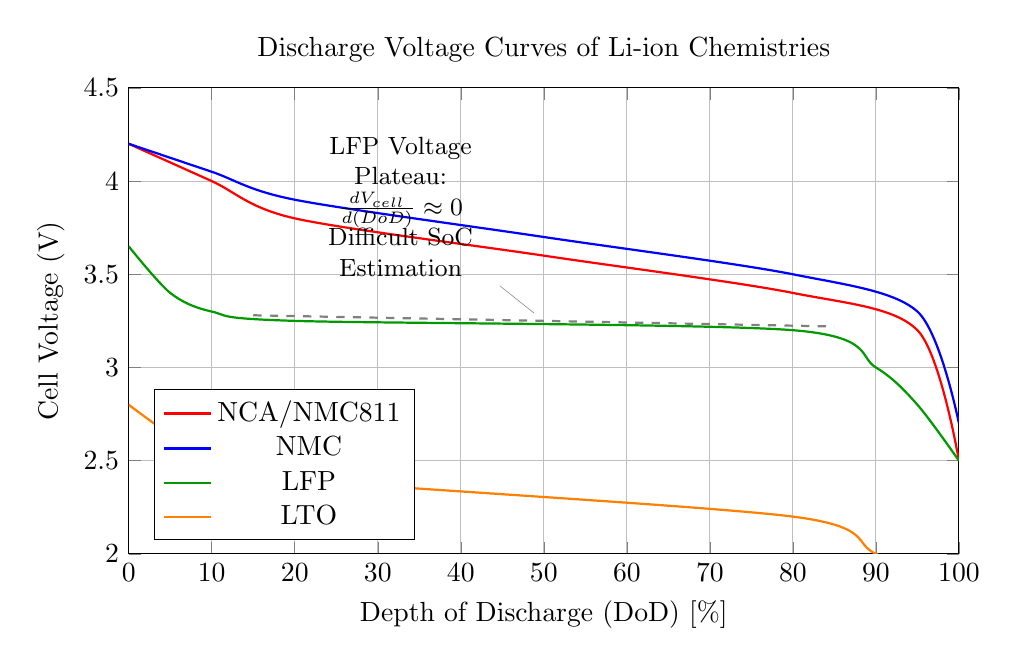
\begin{tikzpicture}
        \begin{axis}[
            title={Discharge Voltage Curves of Li-ion Chemistries},
            xlabel={Depth of Discharge (DoD) [\%]},
            ylabel={Cell Voltage (V)},
            xmin=0, xmax=100,
            ymin=2.0, ymax=4.5,
            grid=major,
            legend pos=south west,
            width=\textwidth,
            height=7.5cm,
        ]
        \addplot[smooth, thick, red] coordinates { (0, 4.2) (10, 4.0) (20, 3.8) (50, 3.6) (80, 3.4) (95, 3.2) (100, 2.5) };
        \addlegendentry{NCA/NMC811}

        \addplot[smooth, thick, blue] coordinates { (0, 4.2) (10, 4.05) (20, 3.9) (50, 3.7) (80, 3.5) (95, 3.3) (100, 2.7) };
        \addlegendentry{NMC}

        \addplot[smooth, thick, green!60!black] coordinates { (0, 3.65) (5, 3.4) (10, 3.3) (20, 3.25) (80, 3.2) (90, 3.0) (95, 2.8) (100, 2.5) };
        \addlegendentry{LFP}
        
        \addplot[smooth, thick, orange] coordinates { (0, 2.8) (10, 2.5) (20, 2.4) (80, 2.2) (90, 2.0) (100, 1.8) };
        \addlegendentry{LTO}

        \draw[dashed, thick, gray] (axis cs:15,3.28) -- (axis cs:85,3.22);
        \node[pin=135:{\parbox{2.5cm}{\centering \small LFP Voltage Plateau: \\ $\frac{dV_{cell}}{d(DoD)} \approx 0$ \\ Difficult SoC Estimation}}] at (axis cs:50,3.25) {};
        \end{axis}
    \end{tikzpicture}
    \caption{Typical discharge voltage curves for various lithium-ion chemistries. The flat profile of LFP makes accurate SoC estimation challenging based on voltage alone\footcite{plett2015battery}.}
    \label{fig:voltage_curves_detailed}
\end{figure}

As shown in Figure \ref{fig:voltage_curves_detailed}, LFP's flat voltage plateau makes it difficult for the BMS to determine the precise SoC in the central part of its operating range. This necessitates periodic full charges to 100\% to recalibrate the system at a point where the voltage curve is steep again, an important operational constraint for V2G control strategies.

\subsection{Comparative Analysis and Safety Considerations}
The trade-offs between chemistries are summarized in Table \ref{tab:chem_comparison_detailed}. Safety is paramount, and the primary risk is thermal runaway. The risk is directly related to the stored energy density ($\Delta E / \Delta m$). A higher energy density means more energy is packed into a smaller mass, which can be released violently if the cell's structure is compromised. Consequently, the critical temperature for initiating thermal runaway is generally lower for higher energy density chemistries. As energy density decreases, the thermal stability increases.

\begin{table}[h!]
\centering
\caption{Comparative analysis of key automotive battery chemistries\footcite{blomgren2017development, wang2012thermal}.}
\label{tab:chem_comparison_detailed}
\resizebox{\textwidth}{!}{%
\begin{tabular}{@{}lccccc@{}}
\toprule
\textbf{Metric} & \textbf{NCA} & \textbf{NMC} & \textbf{LFP} & \textbf{LTO} & \textbf{LCO} \\
\midrule
\textbf{Energy Density (Wh/kg)} & 200 - 260 (Highest) & 150 - 220 (High) & 90 - 160 (Moderate) & 60 - 110 (Low) & 150-200 (High) \\
\textbf{Cycle Life} & 1000 - 2000 & 1000 - 2500 & 2000 - 5000+ & >10,000 & 500 - 1000 \\
\textbf{Safety} & Good & Very Good & Excellent & Excellent & Poor \\
\textbf{Thermal Runaway Temp ($^{\circ}$C)} & $\sim$150 - 180 & $\sim$180 - 210 & $\sim$220 - 270 & >250 & $\sim$150 \\
\bottomrule
\end{tabular}%
}
\end{table}

\subsection{Battery Pack Architecture}
Individual cells are assembled into modules and packs using a series-parallel configuration, denoted as \textbf{XsYp}. 'X' cells in series determine the pack voltage ($V_{pack} = X \cdot V_{cell}$), which is typically 350-400V for modern EVs. 'Y' cells in parallel determine the pack capacity ($C_{pack} = Y \cdot C_{cell}$). While the physical form factor (cylindrical, prismatic, pouch) and BMS design are critical for engineering, our focus remains on the electrochemical degradation influenced by V2G control strategies.